\documentclass[a4paper]{jpconf}
% \bibliographystyle{iopart-num}
\usepackage{amsmath}
\usepackage{citesort}
\usepackage{subfigure}
\usepackage{graphicx}
\graphicspath{{fig/}}
\usepackage{ifpdf}
\ifpdf\usepackage{epstopdf}\fi
\usepackage[export]{adjustbox}

%----------------------------------------------------- 
%\usepackage{soul,ulem,color,xspace,bm}
% Suggest to remove
%\newcommand{\asrm}[1]{{\color{magenta}\sout{#1}}}
% Suggest to insert
%\newcommand{\as}[1]{\color{cyan}#1\xspace\color{black}}
% Suggest to replace
%\newcommand{\asrp}[2]{\asrm{#1} \as{#2}}
% Comment
%\newcommand{\ascm}[1]{{\color{green}\;AS: #1}}
%------------------------------------------------------

\def\apj{ApJ}
\def\mnras{MNRAS}
\def\nat{Nat}
\def\prd{Phys. Rev. D}
\def\araa{ARA\&A}                % "Ann. Rev. Astron. Astrophys."
\def\aap{A\&A}                   % "Astron. Astrophys."
\def\aaps{A\&AS}                 % "Astron. Astrophys. Suppl. Ser."
\def\aj{AJ}                      % "Astron. J."
\def\apjs{ApJS}                  % "Astrophys. J. Suppl. Ser."
\def\pasp{PASP}                  % "Publ. Astron. Soc. Pac."
\def\apjl{ApJ}                   % letter at ApJ
\def\pasj{PASJ}
\def\apss{Astroph. Space Sci.}
\def\aplett{Astroph. Lett}
\def\ssr{Space Sci. Rev.}
\def\aapr{Astron. Astroph. Reviews}
\def\physrep{Phys. Reports}
\def\memsai{Mem. Societa Astronom. Italiana}
\def\jgr{JGR}
\def\jcap{Journal of Cosmology and Astroparticle Physics}

\usepackage{xspace}
\usepackage[dvipsnames]{xcolor}
\usepackage[normalem]{ulem}
% Suggest to remove
\newcommand{\asrm}[1]{{\color{OrangeRed}\sout{#1}}}
% Suggest to insert
\newcommand{\as}[1]{\color{RoyalBlue}#1\xspace\color{black}}
% Suggest to replace
\newcommand{\asrp}[2]{\asrm{#1} \as{#2}}
% Comment
\newcommand{\ascm}[1]{{\color{ForestGreen}#1}}

\begin{document}
	\title{Evaluating MHD parameters of relativistic shock waves with particle-in-cell modeling}
	
	\author{V I Romansky$^{1}$, A M Bykov$^{1,2}$ and S M Osipov$^{1}$}
	
	\address{$^1$ Ioffe Institute, 26 Politekhnicheskaya st., St. Petersburg 194021, Russia}
	\address{$^2$ Peter the Great St. Petersburg Polytechnic University, 29 Politekhnicheskaya st., St. Petersburg 195251, Russia}
	
	\ead{romanskyvadim@gmail.com}
	
	\begin{abstract}
                 Relativistic plasma outflows are observed in gamma-ray burst 
		sources, jets of active galactic nuclei, pulsar wind nebulae and
		supernovae explosions. Magnetohydrodynamical (MHD) shock waves
		inevitably result from interactions of such relativistic outflows with
		the ambient interstellar matter. The widely used single-fluid MHD
		description of relativistic shock waves is the main tool to study the
		global structure of such objects. However, to justify the validity of 
		the global MHD models and to interpret the observed
		emission spectra of space objects with relativistic shocks, a kinetic
		description of electrons, positrons, and ions at microscales is needed. 
		We model a plane relativistic shock propagating  transverse to a regular magnetic field in the electron-ion plasmas with imposed turbulent fluctuations in the shock upstream.   
           Namely we study  the effect of the micro-scale plasma processes on 
		macroscopic parameters of the mildly-relativistic shocks as the adiabatic index
		of the relativistic fluid in the shock downstream. The adiabatic index is a macroscopic parameter of the
		single-fluid MHD models commonly used for shock modeling at much
		longer hydrodynamical scales and it is especially important for the MHD modeling of the mildly-relativistic shocks.
	\end{abstract}
	
	\section{Introduction}
	Relativistic jets and winds are the generic outflows of the relativistic supernovae \cite{2010Natur.463..513S,2007ApJ...667..351W}, the accreting black holes, both suprmassive in the active galactic nucleis  \cite{1984RvMP...56..255B} as well as the stellar masses in the gamma-ray burst sources, microquasars \cite{2019MmSAI..90...57M,1999PhR...314..575P,2014LNP...876.....R} and pulsar wind nebulae \cite{2019MNRAS.488.5690O,2017SSRv..207..235B,2017JPlPh..83e6301K,2019ApJ...876L...8B}. Relativistic shocks can be formed either inside the flow of low or moderate magnetization (the internal shocks) or can be driven by the outflow colliding with the ambient medium (the external shocks). In many cases the relatistivistic shocks in astrophysical objects are collisionless and are often associated with non-equilibrium particle distributions \cite{2012SSRv..173..309B,2015SSRv..191..519S,2017SSRv..207..319P}. They can accelerate particles to ultra-high energies \cite{2009JCAP...11..009L}. On the one hand, the presence of non-maxwellian components with very long equilibration time requires a kinetic description of the shocked flows. The kinetic structure of relativistic shocks can be modelled within the particle-in-cell approach, which allows one to properly account for the electron scale processes and for the density of the displacement current which is important in relativistic plasma flows.  On the other hand, available computer capabilities do not alow one to provide a fully kinetic modelling of the macroscopic astrophysical flows and, therefore, the fluid MHD description based on such macroscopic parameters as the effective adiabatic index of the flow is widely used. Here we discuss an approach allowing to determine the effective adiabatic indexes from the microscopical particle-in-cell modeling of the mildly-relativistic shocks typical for the relativistic supernovae and gamma-ray burst afterglows.   
	
	Relativistic fluid shock dynamics was discussed by Lichnerowicz \cite{1967rhm..book.....L}, Blandford and McKee \cite{Blandford76} and by Emmering and Chevalier\cite{Emmering87}. The relativistic shock jump conditions in the case of a perpendicular shock which is typical for relativisic shocks can be written as:
	\begin{equation}\label{hugoniot}
	[\![\rho u^r]\!] = [\![ (w + \frac{B^2}{4 \pi})u^r u^t]\!] = [\![(w + \frac{B^2}{4 \pi}){u^r}^2 + P + \frac{B^2}{8 \pi}]\!] = [\![\frac{B}{\rho}]\!] = 0
	\end{equation}
	where $u = (u^t,u^r)$ is the velocity four-vector measured in the shock frame, $\rho$ is the proper mass density, $B$ is the magnetic field, $P$ is the pressure in the fluid frame, and $w = \rho c^2 + \frac{\hat{\gamma}}{\hat{\gamma} - 1} P$ is the enthalpy, while $\hat{\gamma}$ is the adiabatic index and the double brackets indicate the jump of the quantities between two sides of the shock.
	
	In the ultra-relativistic limit, the shock velocity $v_{sh}$ and the downstream temperature $T$ can be expressed as, respectively, \cite{Amato2006,2011A&ARv..19...42B}:
	\begin{equation}\label{vshock}
	v_{sh} = \frac{c}{2}\frac{1}{1 + \sigma}\lbrace (\hat{\gamma}(1 + \frac{\sigma}{2})-1) + {\lbrack (\hat{\gamma}(1 + \frac{\sigma}{2})-1)^2 + 4\sigma(1+\sigma)(1 - \frac{\hat{\gamma}}{2})\rbrack}^{\frac{1}{2}} \rbrace,
	\end{equation}
	\begin{equation}\label{temperature}
	T = m c^2 \Gamma \frac{v_{sh}}{c}(1 - \frac{\sigma}{2}\frac{c - v_{sh}}{v_sh}),
	\end{equation}
	Where $\sigma$ is the magnetization and $\Gamma$ is the upstream Lorentz-factor measured in the downstream frame. 
	
	The application of the single fluid formalism requires a correct choice of the adiabatic index $\hat{\gamma}$. For a monoatomic gas it is well-defined: in the classical limit $\hat{\gamma} = \frac{5}{3}$ and in the ultra-relativistic limit $\hat{\gamma} = \frac{4}{3}$. However, in the range between these limits the choice of the value of $\hat{\gamma}$ is not trivial. Moreover, the one-fluid model doesn't take into account for the difference between the temperatures of electrons and protons, while the Coulomb relaxation is slow in relativistic astrophysical plasmas. Two-fluid models require some phenomenological approach to account for the collisionless relaxation of the electron temperature.  Therefore, in this study we used the particle-in-cell approach for modelling of relativistic shock waves in order to address the accuracy of MHD equations and to determine the adiabatic index for various cases. 
	
	
	\section{Numerical setup}
	In this study we performed simulations of a perpendicular relativistic shock  varying the magnetization, Lorentz-factor and the fraction of the turbulent field. 
	The simulation domain is two-dimensional with three-dimensional velocities and fields. To perform such computation we employed the publicly available Tristan-mp code with the explicit numerical scheme developed by Buneman \cite{Buneman93} and  Spitkovsky\cite{Spitkovsky2005}.
	
	A shock wave is initialized in an electron-proton plasma which is flowing into the simulation box through its right boundary and then is reflecting from the super-conducting wall at the left boundary.  The typical simulation parameters are : the initial flow Lorentz factor $\Gamma = 1.5$, the flow magnetization $\sigma = \frac{B^2}{4\pi\Gamma (n_p m_p + n_e m_e) c^2}$ was choosen to be  0.004 and 0.0004  (in the turbulent case $B^2$ is the mean square field). The dimensionless thermal energy $\Delta \gamma = \frac{k T}{m_p c^2}$ is equal to $10^{-4}$ and the electron mass is increased up to $m_e = \frac{m_p}{100}$. The size of the simulation box along the $x$ axis is $L_x = 30000\frac{c}{\omega_p}$ and in the transverse direction $L_y = 400\frac{c}{\omega_p}$, where $\omega_p = \sqrt{\frac{4\pi q^2 n}{\Gamma m_e}}$ is the plasma frequency. These scales correspond to $150000$ and $2000$ grid points in $x$ and $y$ directions, respectively. For 3d setup transverse sizes are reduced to $40$ grid points. Also, $2000$ grid points correspond to approximately $10$ gyroradii of the upstream protons.
	In simulations with turbulent fields, we initialized it as  summ of harmonic modes with Kolmogorov's spectum, as described in detail in\cite{Romansky2019}. The ratio of the energy density of the turbulent field to the total magnetic energy density is denoted as $\eta$ , which varied from 0 percent to 90 percent in our simulations. The regular magnetic field is normal to the $x$ axis and is rotated by the angle $\phi$ about $x$ axis: the value $\phi = 0$ corresponds to the out-of-plane orientation of magnetic field and $\phi = 90$ corresponds to the in-plane orientation.
	
	
	
	\section{Results}
	We used several parameter sets, listed in table \ref{setups}, with different magnetization, Lorentz-factors and the fraction of turbulent field. Also, we investigated differences between 2D and 3D cases.
	\renewcommand{\arraystretch}{1.1}
	\begin{table}[h!]
		\label{setups}
		\caption{Parameters of different setups. }
		\begin{center}
			\begin{tabular}{|c | c| c| c| c| c| c| c| c| c|}
				\hline
				Setup & $\phi$ & $\sigma$ & $\Gamma$ & $\eta$ & $\frac{v_{sh}}{c}$ & $\hat{\gamma}$ & $T \ 10^{12} K$ & $T_p\ 10^{12}K$ & $T_e \ 10^{12}K$\\
				\hline
				reg1  & 0 & 0.004 & 1.5 & 0 & 0.355 & 1.51 & 3.5 & 2.5 & 0.23\\
				reg2  & 90 & 0.004 & 1.5 & 0 & 0.240 & 1.53 & 2.9 & 2.2 & 0.28\\
				reg3 & 0 & 0.0004 & 1.5 & 0 & 0.339 & 1.52 & 3.4 &2.4 & 0.38\\
				reg4  & 90 & 0.0004 & 1.5 & 0 & 0.228 & 1.53 & 2.8 &1.7 & 0.37\\
				turb1  & 0 & 0.004 & 1.5 & 90 & 0.309 & 1.52 & 3.3 & 2.1 & 0.41\\
				turb2  & 0 & 0.004 & 1.5 & 30 & 0.348 & 1.51 & 3.5 & 2.4 & 0.35\\
				gam1  & 0 & 0.004 & 2 & 0 & 0.412 & 1.46 & 6.3 & 4.2 & 0.62\\
				gam2  & 0 & 0.004 & 5 & 0 & 0.479 & 1.39 & 20.5 & 7.3 & 11.0\\
				gam3  & 0 & 0.004 & 10 & 0 & 0.504 & 1.36 & 42.6 & 16.8 & 21.3\\
				reg3d & 0 & 0.004 & 1.5 & 0 & 0.313 & 1.52 & 3.3 & 3.0 & 0.21\\
				
				\hline
			\end{tabular}
		\end{center}
	\end{table}
	
	Using the density profiles of the simulated shock waves, we determined magnetohydrodynamic parameters of plasma, solving the jump conditions (\ref{hugoniot}). The density averaged in transversal directions has clear jump as shown in figures \ref{density_noturb} and \ref{density_turb}, which is indicating the position of the shock front. So we can evaluate the shock velocity from results of simulations, and then solve jump conditions for the adiabatic index and the downstream temperature, using the iterative method. 
	
	\begin{figure}[h!]
		\centering
		\begin{minipage}{0.49\textwidth}
			\centering
			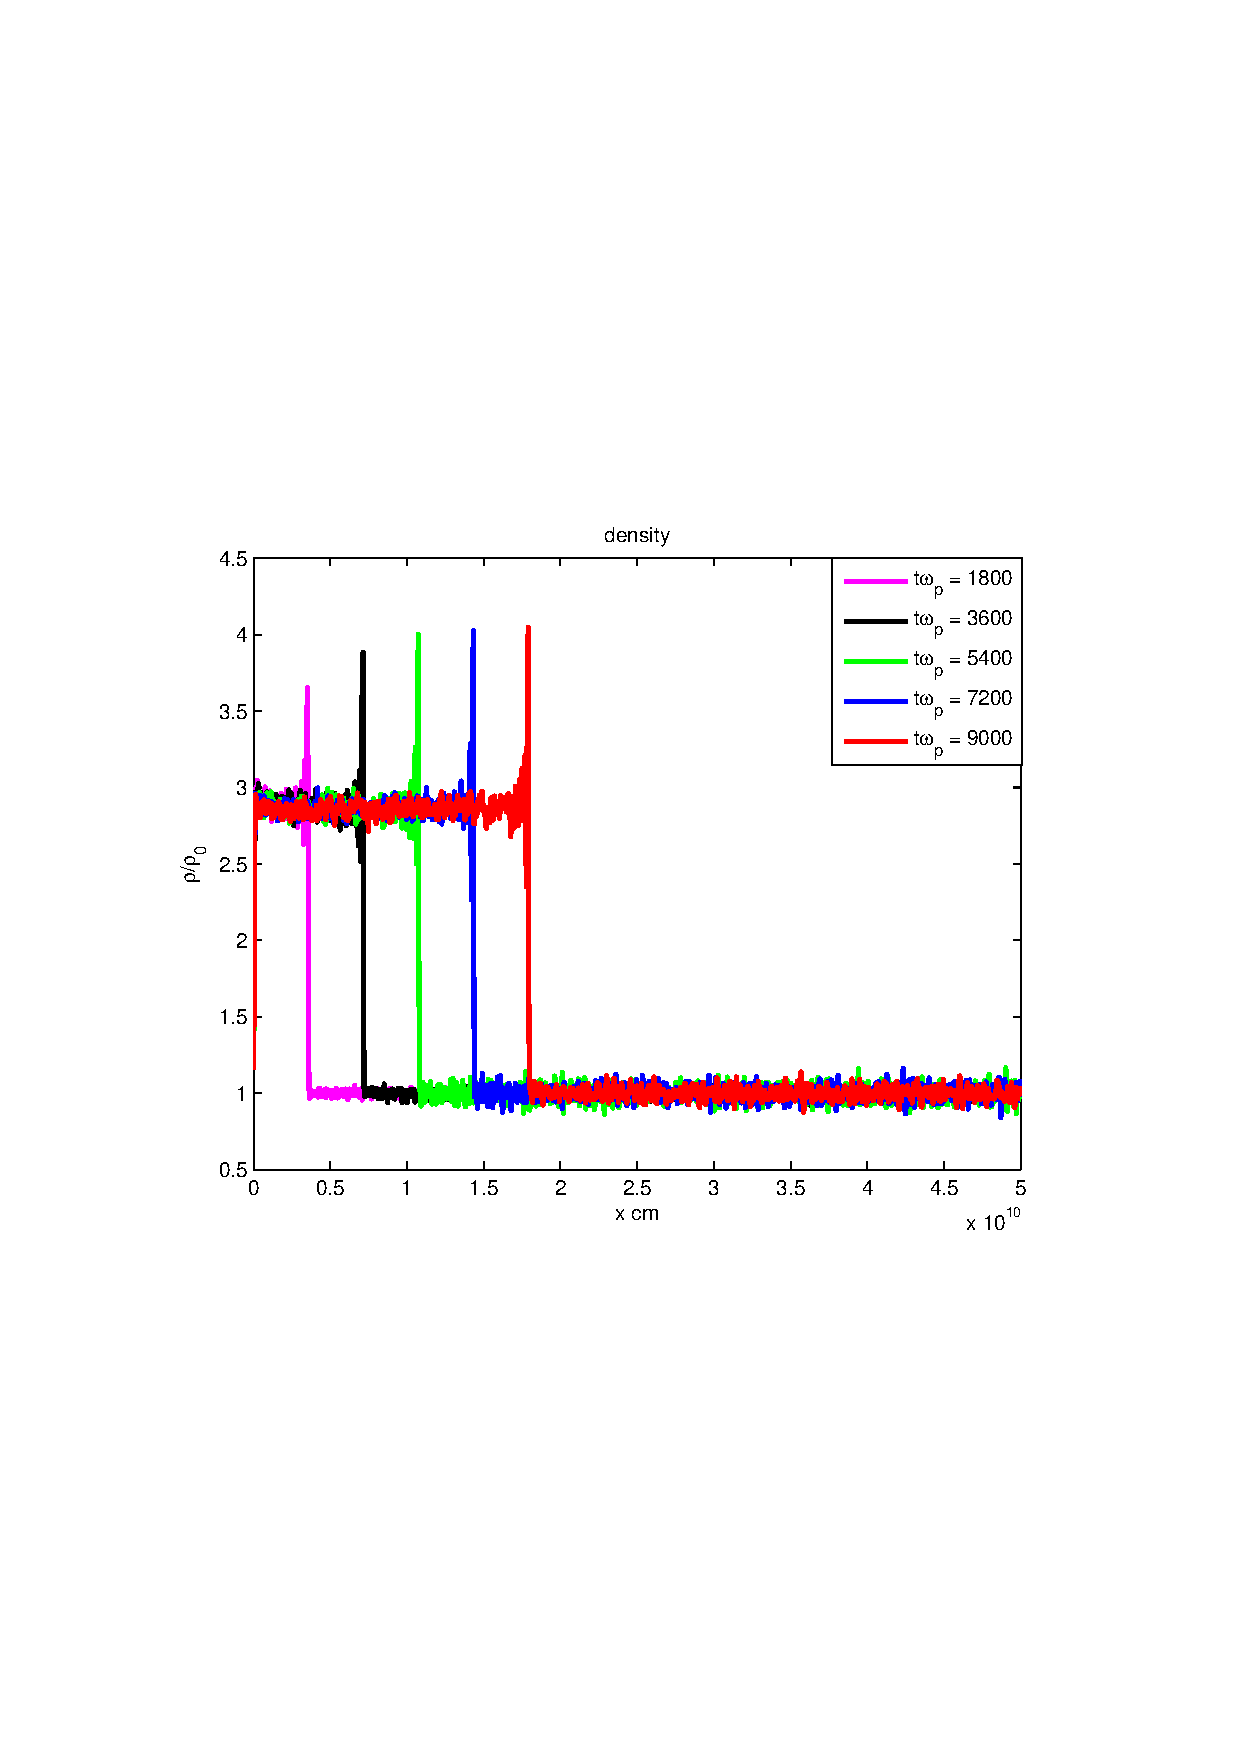
\includegraphics[width=0.98\textwidth]{fig/density_noturb.png} 
			\caption{Density profile of a shock wave in a medium with a regular field, averaged through the transversal dimensions, setup reg1.}
			\label{density_noturb}
		\end{minipage}\hfill
		\begin{minipage}{0.49\textwidth}
			\centering
			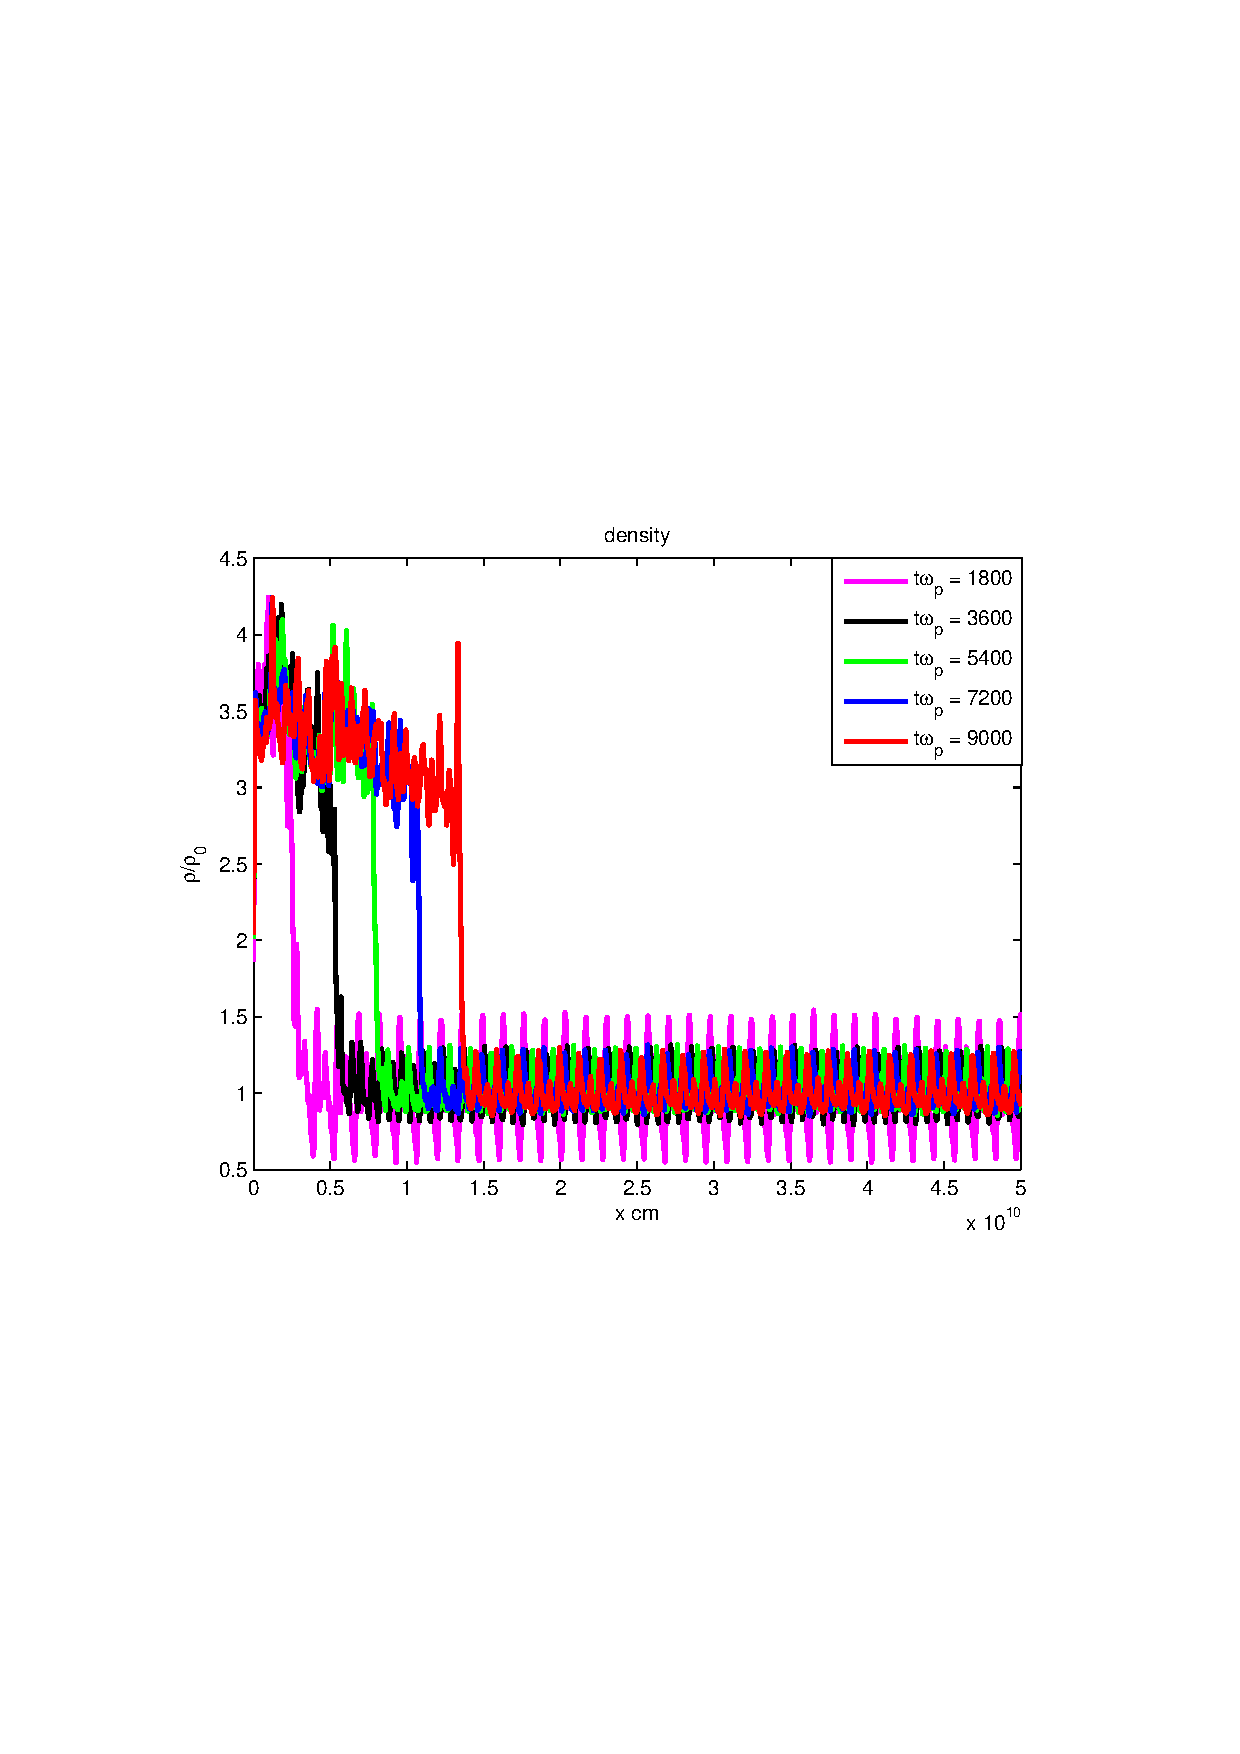
\includegraphics[width=0.98\textwidth]{fig/density_turb.png} 
			\caption{Density profile of a shock wave in a turbulent medium, averaged through the transversal dimensions, setup turb1.}
			\label{density_turb}
		\end{minipage}
	\end{figure}
	
	Evaluation of shock front coordinates, which we have determined as a point where  the density is two times larger than the density observed far upstream, at different time steps shows that the shock front velocity is constant in time up to a high accuracy, see figure \ref{shock_x}. Also, it shows, that the shock front velocity decreases with the decreasing magnetization, and, consequently, the adiabatic index does not remain constant. The shock slows down with the increasing turbulent field energy and it requires significant decrease of the adiabatic index. It can be explained by the appearence of new degrees of freedom related to magnetic field oscillations. Obviously, the shock front is faster for higher values of the upstream Lorentz-factor, and the adiabatic index  converges to the value $4/3$ which is the ultra-relativistic limit. For Lorentz-factors less then 10, $\hat{\gamma}$ is significantly higher than the limiting value. 
	
	
	\begin{figure}[h!]
		\centering
		\includegraphics[width=0.64\textwidth]{fig/shock_x.png} 
		\caption{Evolution of the shock front position for various parameter sets.}
		\label{shock_x}
	\end{figure}
	
	Distributions of particles significantly vary through the x coordinate, and in figure \ref{points} we show the distribution of electrons at different distances from shock front, measured in proton gyroradius $r_g$. Positive distances correspond to upstream region and negative to downstream. As one can see, for distances more than $6 r_g$ in the downstream distribution does not depend on coordinate.  We obtained the temperatures of protons and electrons by fitting their distibutions in far downstream with Maxwell-Juttner function, via minimization of the functional $f(T) = \int_{0}^{p_{max}} (F(p) - F_{m}(p,T))^2dp$ by temperature, where $F(p)$ is the electron or proton distribution derived from the simulation, $F_{m}(p,T)$ is the Maxwell-Juttner function with temperature $T$ and $p_{max}$ is the momentum for which the distributioin becomes non-thermal. Obtained temperature has rather week dependence on choice of $p_{max}$. Such evaluation of the downstream temperature is possible even in the cases of strong non-thermal tail, as shown in figure \ref{temp_fit}.
	
	\begin{figure}[h!]
		\centering
		\includegraphics[width=0.64\textwidth]{fig/electrons_at_points.png} 
		\caption{The distribution functions of electrons at different positions in the shock vicinity (indicated at the insert) within the simulation box for the  turbulent parameter set (turb1). Note that the strong departures from the Maxwell-Juttner distributions and the formation of the non-thermal tails are due to the presence of the external turbulence in the shock upstream.}
		\label{points}
	\end{figure}
	
	\begin{figure}[h!]
		\centering
		\includegraphics[width=0.64\textwidth]{fig/temperature_fit.png} 
		\caption{The simulated distribution functions of electrons at far downstream. The red curve is for the shock propagating transverse to a regular magnetic field. The green curve is for the case of the turbulent upstream magnetic field (the turb1 parameter set). The Maxwell-Juttner fits for the both distributions are shown in the blue and black curves respectively.}
		\label{temp_fit}
	\end{figure}
	
	An analysis of the distribution functions shows that the temperatures of protons and electrons are much smaller than predicted by jump conditions (\ref{hugoniot}). It means that magnetohydrodynamical formalism is not sufficient for the description of downstream temperatures of a relativistic shock wave. One can notice that the ratio of temperature of protons to the temperatures of electrons is not constant: it is close to $\sqrt{\frac{m_p}{m_e}}$ at low Lorenz-factors and decreases down to $1$ at higher ones. Turbulence also has a strong influence on the temperatures, as it makes electrons much hotter, while the protons become colder. 
	
	Finally, a comparison of the results obtained using 2D and 3D setups with the same parameters (setups reg1, reg2 and reg3d) reveals that the differences in results depend on orientation of magnetic field in 2D simulations. For out-of plane orientation these differences are noticeable, but not crucial - temperature and shock velocity differs in 2D and 3D setups by less than on 10 percent. This means that 2D simulations are appropriate for modeling of relativistic collisionless shock waves in magnetized plasmas. 
	
	\section{Conclusions}
	
	Particle-in-cell simulations have been used to derive effective macroscopic parameters of relativistic shocks in space plasmas. The effective adiabatic index and electron temperatures are two important parameters required to supplement large-scale single-fluid magneto-hydrodynamic simulations of processes in astrophysical plasmas. The adiabatic indexes for the downstream flow derived with PiC method are summarized in Table 1 and can be used for MHD modeling of relativistic
	supernovae. Further modelling is needed to study the dependence of these two parameters on the initial conditions which, reflect the presence of MHD large-scale turbulence in the stellar wind of the progenitor massive star upstream of the  mildly-relativistic shock of the supernova. 
	
	\ack
	V I Romansky and A M Bykov acknowledge a support from RSF grant 16-12-10225.
	Results of the work were obtained using computational resources of Peter the Great Saint-Petersburg Polytechnic University Supercomputing Center (http://scc.spbstu.ru)
	
	\section*{References}
	% \bibliographystyle{apalike}
	\bibliographystyle{iopart-num}

	\bibliography{bibliogr}
\end{document}